\documentclass{sigchi}
% Use this command to override the default ACM copyright statement (e.g. for preprints). 
% Consult the conference website for the camera-ready copyright statement.


%% EXAMPLE BEGIN -- HOW TO OVERRIDE THE DEFAULT COPYRIGHT STRIP -- (July 22, 2013 - Paul Baumann)
% \toappear{Permission to make digital or hard copies of all or part of this work for personal or classroom use is 	granted without fee provided that copies are not made or distributed for profit or commercial advantage and that copies bear this notice and the full citation on the first page. Copyrights for components of this work owned by others than ACM must be honored. Abstracting with credit is permitted. To copy otherwise, or republish, to post on servers or to redistribute to lists, requires prior specific permission and/or a fee. Request permissions from permissions@acm.org. \\
% {\emph{CHI'14}}, April 26--May 1, 2014, Toronto, Canada. \\
% Copyright \copyright~2014 ACM ISBN/14/04...\$15.00. \\
% DOI string from ACM form confirmation}
%% EXAMPLE END -- HOW TO OVERRIDE THE DEFAULT COPYRIGHT STRIP -- (July 22, 2013 - Paul Baumann)


% Arabic page numbers for submission. 
% Remove this line to eliminate page numbers for the camera ready copy
\pagenumbering{arabic}


% Load basic packages
\usepackage{balance}  % to better equalize the last page
\usepackage{graphics} % for EPS, load graphicx instead
\usepackage{times}    % comment if you want LaTeX's default font
\usepackage{url}      % llt: nicely formatted URLs
\usepackage{verbatim}
\usepackage{tabularx}
% llt: Define a global style for URLs, rather that the default one
\makeatletter
\def\url@leostyle{%
  \@ifundefined{selectfont}{\def\UrlFont{\sf}}{\def\UrlFont{\small\bf\ttfamily}}}
\makeatother
\urlstyle{leo}


% To make various LaTeX processors do the right thing with page size.
\def\pprw{8.5in}
\def\pprh{11in}
\special{papersize=\pprw,\pprh}
\setlength{\paperwidth}{\pprw}
\setlength{\paperheight}{\pprh}
\setlength{\pdfpagewidth}{\pprw}
\setlength{\pdfpageheight}{\pprh}

% Make sure hyperref comes last of your loaded packages, 
% to give it a fighting chance of not being over-written, 
% since its job is to redefine many LaTeX commands.
\usepackage[pdftex]{hyperref}
\hypersetup{
pdftitle={SIGCHI Conference Proceedings Format},
pdfauthor={LaTeX},
pdfkeywords={SIGCHI, proceedings, archival format},
bookmarksnumbered,
pdfstartview={FitH},
colorlinks,
citecolor=black,
filecolor=black,
linkcolor=black,
urlcolor=black,
breaklinks=true,
}

% create a shortcut to typeset table headings
\newcommand\tabhead[1]{\small\textbf{#1}}


% End of preamble. Here it comes the document.
\begin{document}

\title{Voice Interfaces for Visually Impaired and Low-Literate Communities in the Developing World}

\numberofauthors{2}
\author{
  \alignauthor Aditya Vashistha\\
    \email{adityav@cs.washington.edu}\\
   \alignauthor Sam Sudar\\
    \email{sudars@cs.washington.edu}\\}

\maketitle

\begin{comment}

\begin{abstract}
Millions of people cannot access services using conventional graphical user
interfaces. These users include the visually impaired, the low-literate,
speakers of tribal languages without font support, and those without access to
computers or mobile devices. Interactive voice response (IVR) systems provide a
way to interact with users without the need for graphics. Callers are read
options and use the keypad to navigate the content, lowering the barriers for
access and providing the opportunity for engagement. Current IVR systems
provide a wide spectrum of services, including health information, citizen
journalism, and social media. However, little work has been done to inform
the organization of IVR content. We compare list, shallow and deepr hierarchies
to organize content in an IVR system, expanding on similar work that has
focused on graphical user interfaces. We find that both flat lists and deep
hierarchies are inappropriate, and that shallow hierarchies create a more
effective IVR structure.
\end{abstract}

\keywords{
	Guides; instructions; author's kit; conference publications;
	keywords should be separated by a semi-colon.
	\textcolor{red}{Mandatory section to be included in your final version.}
}

\category{H.5.m.}{Information Interfaces and Presentation (e.g. HCI)}{Miscellaneous}

See: \url{http://www.acm.org/about/class/1998/}
for more information and the full list of ACM classifiers
and descriptors. 
\textcolor{red}{Mandatory section to be included in your
final version. On the submission page only the classifiers'
letter-number combination will need to be entered.}

\end{comment}

\section{Introduction}
According to the World Health Organization, 285 Million people in the world are visually impaired (VI) and 90\% of them live in developing countries \cite{WHO2013}. VI people in developing countries have limited access to assistive technologies because of various socio-economic, device-related and network related constraints. In India, only
5\% of all mobile phone subscribers own a smartphone \cite{Mary2013}. The remaining 95\% use a basic or feature phone;these typically have only one inbuilt assistive tool for VI people, a speaking clock. Lack of screen readers on these devices and tactile interfaces force VI users to access information and provide data using voice based communication on their phones. 

The literacy rate in most developing countries is quite low. For example, 26\% people in India are illiterate and the rate of functional illiteracy is surprisingly high. Even in a developed country like US where the claimed literacy rate is 99\%, around 20\% of adults are functionally illiterate. Thus, text based interfaces are out of reach of sighted low-literate communities as well. In India, there are millions of speakers of tribal languages like Kui, Kurukh, Gondi. However, the font support for many tribal languages is still non-existent. Thus many literate tribal people also use voice medium for producing and accessing information. The limited usage of computing devices like smartphone, tablet and desktop limits adoption of graphical user interfaces designed for low-literate low-income communities. As a result, these communities also use their basic or feature phones to access informational services on the voice channel.

In recent years, various researchers and practitioners have used Interactive Voice Response (IVR) systems to provide health information, citizen journalism, educational services, feedback channels, data collection systems, social media platform etc. for low-literate marginalized communities. IVR systems have also been used as a means to provide information to and collect data from VI people with low socio-economic status. Though there are a lot of success stories of organizations appropriating IVR systems for societal development, there are a few challenges that impede the sustainable usage of such systems. The first challenge is the high cost of calls for accessing information. The second challenge is inefficient audio content management. Hierarchical call tress are used in IVR system to structure the information much like a menu in graphical user interfaces. However, auditory interfaces are quite different from textual and graphical interfaces. Voice interfaces force users to access information sequentially, which results in frustration, high cost, and low-usability. Moreover, searching and indexing audio recordings on an IVR system are non-trivial operations because of unavailability of high efficacy speech recognition engines for resource constrained languages spoken in developing countries. Because of the above reasons, concentrated efforts are needed for accurate and swift retrieval of information to decrease the time required by callers and to increase usability. 

Our aim is to understand ways in which voice interfaces on an IVR platform can be organized so as to optimize information seeking time, information absorption and call duration. Through this project, we are evaluating expressiveness and effectiveness of various voice interface designs for providing information to low-literate and VI communities. Our research will answer the following research questions:

\begin{itemize}
\item Is hierarchical voice menu better than a linear list?
\item How many number of items in a linear list are acceptable?
\item Is shallow hierarchy better than deep hierarchy?
\item How deep or shallow the hierarchy should be?
\item How abstraction capabilities, literacy level and prior exposure to IVR impacts different designs of voice user interfaces? 
\end{itemize}


\section{Related Work}

\subsection{Interfaces for Low-Literate People}
A lot of work has been done in designing user interfaces for low-literate low-income communities in the developing world. Most of the work explore usage of graphical interfaces \cite{Grisedale1997,Medhi2011a,Medhi2008,Ghosh2003} and auditory interfaces \cite{Cuendet2013,Agarwal2010,Mudliar2013} for collecting data and providing information to marginalized low-literate communities. Various researchers have explored challenges faced by literate users while accessing hierarchical menus \cite{Allen1983,Chaudry2012}. However, the most relevant work to our project is done by Medhi et. al. where they presented how limited education affect hierarchical user interface navigation on desktops and mobile phones \cite{Medhi2013a,Medhi2013b}. Medhi measured the textual literacy level, and abstract reasoning level for low-income low-literate people in India. The participants were then asked to find items from graphical user interfaces consisting of a linear list, shallow, and deep hierarchy. Medhi found that low-income low-literate communities performed best when navigating a linear structure on both desktops as well as mobile phones.

\subsection{Interfaces for VI People}
Although VI people can use screen readers to access information on the Internet, this requires a computer/smartphone, expensive screen reader software, and an Internet connection which is beyond the reach of the majority of the low-income VI people in the developing world \cite{McCarthy2012}. Our parallel research (under review in MobileHCI 2014) has demonstrated that many low-income VI people do not use screen reader software but use alternate information and communication tools for accessing information. Many participants of the study indicated using IVR systems for accessing educational and entertainment content. Some work has also been done to augment or replace visual menus on desktop, mobile phone and other electronic gadgets like music player for improved usability and accessibility \cite{Yalla2008,Zhao2007,Jeon2012}. However, no work has been done yet to understand the trade-offs between using list and different kind of hierarchical interfaces to organize information in IVR systems.

\subsection{IVR Design Guidelines}
Various researchers have provided design guidelines to create effective IVR systems and decrease cognitive load on the callers	 \cite{Ndwe2008,Suhm2008,MSDNSpeech,Halstead-Nussloch1989}. However, a few guidelines focus on the breadth and depth of navigation IVR trees. Various researchers have investigated deep and shallow hierarchies in IVR systems for high-literate users in the developed world \cite{Huguenard1997,Virzi1997,Commarford2008}. For instance, Commarford et.al. compared deep and shallow IVR hierarchies and concluded that deep hierarchies take longer to navigate and have high cognitive load \cite{Commarford2008}. However, the participants of the study were undergraduate students with at least 3-months of email experience and were based out in United States. 

Researchers have also studies various facets of IVR systems to improve information consumption and production by low-income low-literate population in the developing world. Chakraborty et.al. has provided design guidelines for creating IVR surveys for low-literate low-income marginalized communities in India \cite{Chakraborty2013}. Kummamuru et.al. has analyzed the relationship between cognitive load and various navigational factors like breadth, depth, type of information, and numerical order \cite{Kummamuru2012}. They asked semi-literate participants in India to find job information from a synthetic IVR job repository. Each participant had to complete eight tasks. The tasks were designed such that the impact of depth, breadth and other parameters can be measured on the cognitive load. They found that the time to choose right option decreases as the breadth and depth increases. This is because practice and learning effects impact the time taken to navigate the depth. Moreover, cognitive load is high while listening to the first few options in the breadth and thus, the navigation time is lesser for later options in the breadth. The biggest weakness of the paper is the absence of direct comparisons between linear lists, shallow hierarchies and deep hierarchies.

To the best of our knowledge, our work will be the first to directly compare linear list, shallow hierarchy and deep hierarchy for maximizing information absorption by low-literate, low-income communities and visually impaired people in India. 

\section{Design}
We have conducted 3 between-subjects experiment design to compare three designs of IVR interfaces: linear list, shallow hierarchical interface, and deep hierarchical interface. We have used \textit{Household items} dataset used by researchers for comparing performance of low-literate communities on list, shallow and deep hierarchy graphical user interfaces \cite{Medhi2013a,Medhi2013b}. We chose the same dataset in order to directly compare our finding with the findings for graphical visualization. The list voice user interface is a sequential list of the household items. Shallow hierarchical voice user interface has a branching factor of five and the depth of the tree is two (see figure 1). The branching factor for deep hierarchical interface is up to four, and the depth of the tree is four (see figure 2). We have implemented the design structures in VoiceXML using Voxeo Prophecy and IVR Junction \cite{Vashistha}. We have also logged user's interaction with the IVR system while performing tasks to review the actions user took while performing the tasks.

\begin{figure}[!h]
\centering
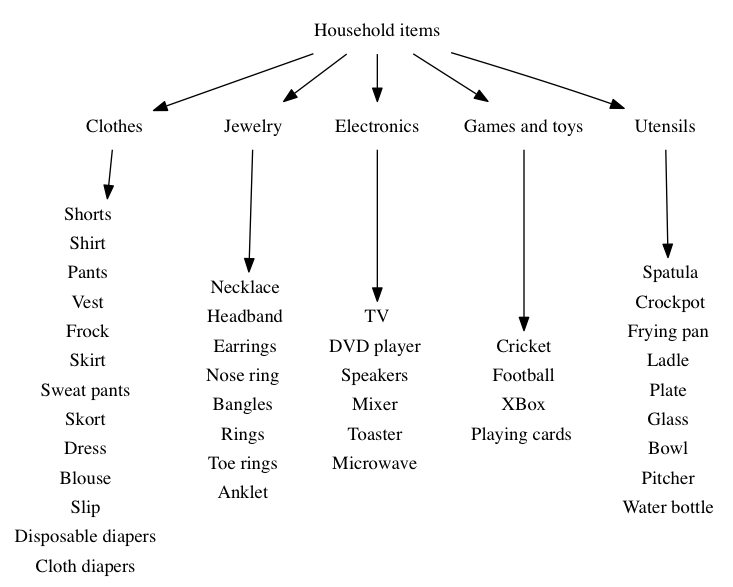
\includegraphics[width=0.9\columnwidth]{ShallowHierarchy}
\caption{Shallow hierarchy arrangement of household items}
\label{fig: Figure1}
\end{figure}

\begin{figure}[!h]
\centering
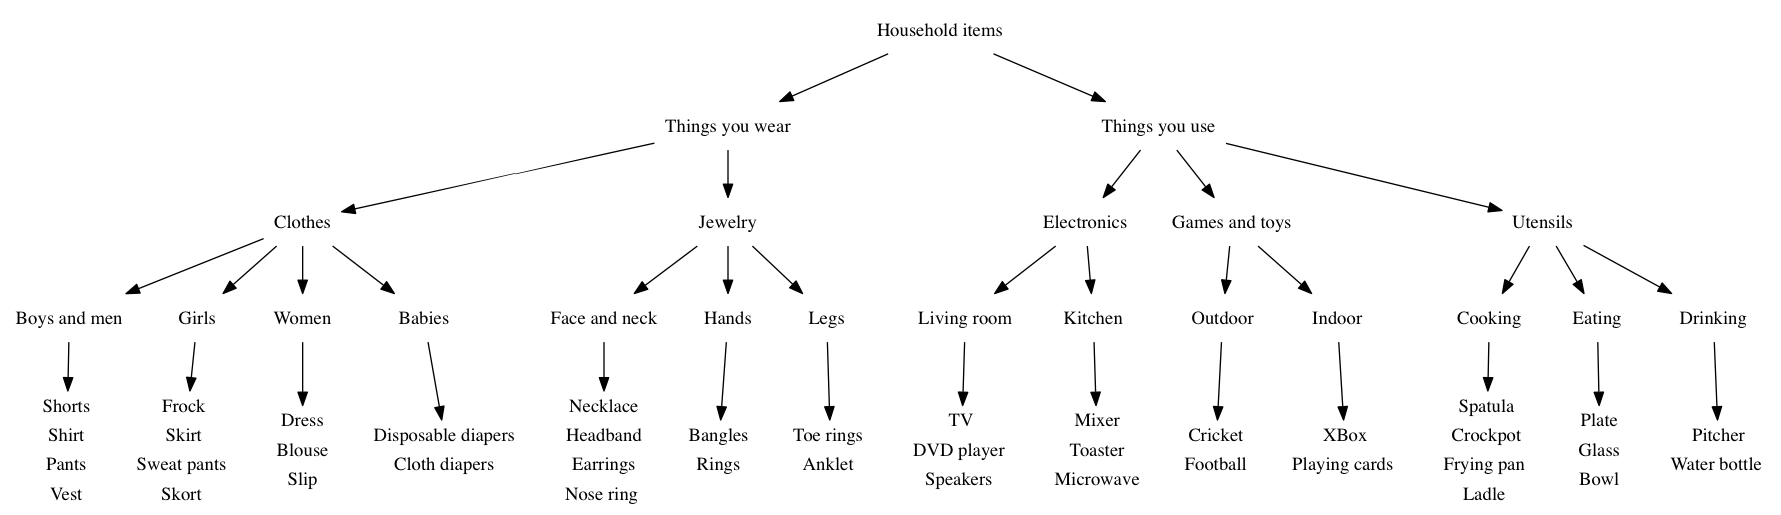
\includegraphics[width=0.9\columnwidth]{DeepHierarchy}
\caption{Deep hierarchy arrangement of household items}
\label{fig: Figure2}
\end{figure}

Participants were randomly divided into 3 groups where each group contained equal number of participants. Each participant performed five tasks, one after another. Each task consisted of selecting a target item from the assigned design structure. All participants searched for five target items (Shirt, Blouse, Rings, Football, and Plate) in the same order. We did not randomize the tasks for participants to ensure that the learning effects for each participant is same. We selected two easy tasks (\textit{find Shirt, Blouse}), one task of intermediate difficulty (\textit{find Rings}), and two complex tasks (\textit{find Football, Plate}). The comparative complexity of performing a particular task (say \textit{find Rings}) across different hierarchies is same as the number of hops required to reach the target item (excluding navigational prompts) in a brute force manner is same for each design structure.  

\section{Evaluation}
We recruited 18 participants (12 Male, 6 Female) to evaluate three design structure. All the participants were either students or employee of the Computer Science department of the University of Washington. The average age of the participants was 26.7 years (max=52, min=19) and the average education level was masters. Sixteen participants were heavy users and two were moderate users of IVR systems. None of the participant was visually impaired. 

Before beginning the task, participants were shown a demo task where they had to find an item from the randomly assigned design structure. We used a different dataset (animal and birds) to illustrate the task and design structure to participants. Participants were allowed to perform demo task at most two times before starting the actual experimental task. We also observed participants while they were performing the task for understanding the challenges they faced while navigating design structures. After completing the task, we interviewed participants to collect demographic information. Participants also completed a short survey where they rated their performance, frustration, and physical, temporal and mental efforts exuded while performing the tasks. 

The following criteria were used for evaluating information absorption and swiftness in navigating the design structures:
\begin{itemize}
\item Task completion rate
\item Task correctness
\item Average task completion time
\end{itemize}

\textbf{TO DO}
\begin{itemize}
\item Tell the overall correctness and time taken for List, Deep and Shallow. 
\item Graphs: Box plots of time taken for all tasks in List, Shallow and Deep. Graphs created by Aditya in poster with error bars. Graphs plotted by Sam depicting results of NASA study. 
\item explain the graphs
\end{itemize}

\section{Analysis and Recommendation}
\textbf{TO DO}
\begin{itemize}
\item What are the salient observations? 
\item What did you find out - Try to rationally explain the findings
\item how is it different from the hierarchical comparisons done for graphical interfaces for US population? Why? (Read literature survey, some people have done the same for graphical interfaces where test subjects were university students) 
\item tell problems in our hierarchy - ambiguity in Rings, Shirt, Pants
\item tell participants frustration, confusion while navigating hierarchies
\item tell how two participants while navigating deep hierarchy chose a wrong path but then figured it out and selected the right option eventually. 
\end{itemize}


\textbf{Sam's recommendations}

\begin{itemize}
\item  Lists have a wide distribution of completion times and are frustrating to users
\item Hierarchies provide the opportunity for performance feedback while completing the task
\item Real world hierarchies will have classification ambiguity. Shallow hierarchies limit the impact of hierarchy decisions and keep the choices intuitive for a broader group of users
\item Shallow hierarchies outperform the other two categories in frustration and performance
\item Use a shallow hierarchy
\end{itemize}

\textbf{Aditya's recommendations}
\begin{itemize}
\item List of size 9 is better than deep or shallow of 9 items because time taken to traverse a list of this size is less than navigating hierarchical structure
\item Within deep and shallow hierarchies, recommend using the list of items less than 9 items at the last level 
\end{itemize}



\section{Future Work}
We will recruit visually impaired people, and low-literate people from India to participate in our study. We will work with a local organization in Madhya Pradesh to get access to the marginalized communities. We will measure the recruited participants on three variables:
\begin{itemize}
\item Literacy level (low, medium/high)
\item Cognitive skills (low, medium/high)
\item Familiarity to IVR usage (limited, medium/high)
\end{itemize}

Previous research has indicated strong correlation between literacy level and cognitive skills \cite{Reis2001,Medhi2013a}. Thus, we will group participants in 4 groups on the basis of the level of cognitive skills and familiarity with IVR:

\begin{itemize}
\item People with low cognitive skills and limited IVR experience
\item People with low cognitive skills and medium/high IVR experience
\item People with medium/high cognitive skills and limited IVR experience
\item People with medium/high cognitive skills and medium/high IVR experience
\end{itemize}

We will also measure \textbf{(TO DO)}:  \textbf{Add Sam's point here}

\begin{itemize}
\item Impact of hierarchy appropriateness on usability
\item Items that are more easily categorizable (e.g. animal species broken by taxa)
\item Greater than 40 items--when does a shallow hierarchy become insufficient?
\item Is shallow preferable to deep simply because there were fewer questions asked? What if shallow was a single hop but had 15 intermediate questions? Would it still be found preferable? Perhaps users don't like having to stay alert and make decision in the hierarchy
\item What is the ideal number of items in a list at any given point? E.g. some users seemed confused by having to press two buttons on the keypad
\item What is the ideal number of questions in intermediary levels? E.g. perhaps a deep binary tree would out perform our deep tree with a variable branching factor
\item Compare different shallow and deep hierarchies with proportional branching factor and depth of the tree. In our experiment, the ratio of depth was 2: 4 for shallow and deep. It would be great proportions like 4: 8 and 3:6 to understand which is better among deep and shallow. 
\end{itemize}

\section{Conclusion}
\textbf{TO DO}

WRITE THE CONCLUSION

\section{Miscellaneous To-DOs}
\begin{itemize}
\item GitHub page for the project
\item Upload paper and other artifacts in the repository. 
\end{itemize}





% Balancing columns in a ref list is a bit of a pain because you
% either use a hack like flushend or balance, or manually insert
% a column break.  http://www.tex.ac.uk/cgi-bin/texfaq2html?label=balance
% multicols doesn't work because we're already in two-column mode,
% and flushend isn't awesome, so I choose balance.  See this
% for more info: http://cs.brown.edu/system/software/latex/doc/balance.pdf
%
% Note that in a perfect world balance wants to be in the first
% column of the last page.
%
% If balance doesn't work for you, you can remove that and
% hard-code a column break into the bbl file right before you
% submit:
%
% http://stackoverflow.com/questions/2149854/how-to-manually-equalize-columns-
% in-an-ieee-paper-if-using-bibtex
%
% Or, just remove \balance and give up on balancing the last page.
%
\balance

\bibliographystyle{acm-sigchi}
\bibliography{library}
\end{document}
